\chapter{Flow Matching}
\label{chap:flow}

Le \emph{Conditional Flow Matching} (Lipman et al., 2023) \cite{lipman2023flow} propose une
reformulation du même principe que la diffusion — transformer progressivement du bruit en donnée — mais
en des termes plus directs, empruntés à la théorie des équations différentielles ordinaires (ODE)
plutôt qu'aux chaînes de Markov gaussiennes.

\section{Des chemins discrets aux chemins continus}

Le DDPM construit implicitement un chemin \emph{stochastique} entre $x_0$ (donnée) et $x_T$ (bruit),
en $T$ pas discrets, chacun ajoutant un peu de bruit aléatoire. Le flow matching part d'une idée plus
simple : et si on définissait directement un chemin \textbf{déterministe et continu} entre les deux ?

\begin{definition}[Chemin d'interpolation linéaire]
Pour $t \in [0, 1]$ continu (notez le changement de convention par rapport au DDPM : ici $t=0$ est la
donnée et $t=1$ est le bruit), on définit :
\begin{equation}
    \label{eq:flow-interp}
    x_t = (1-t)\, x_0 + t\, x_1, \qquad x_0 \sim p_{\text{data}}, \quad x_1 \sim \mathcal{N}(0, I)
\end{equation}
\end{definition}

C'est un simple segment de droite dans l'espace des images : à $t=0$ on est exactement sur la donnée,
à $t=1$ exactement sur le bruit, et entre les deux, un mélange linéaire.

\begin{figure}[h]
\centering
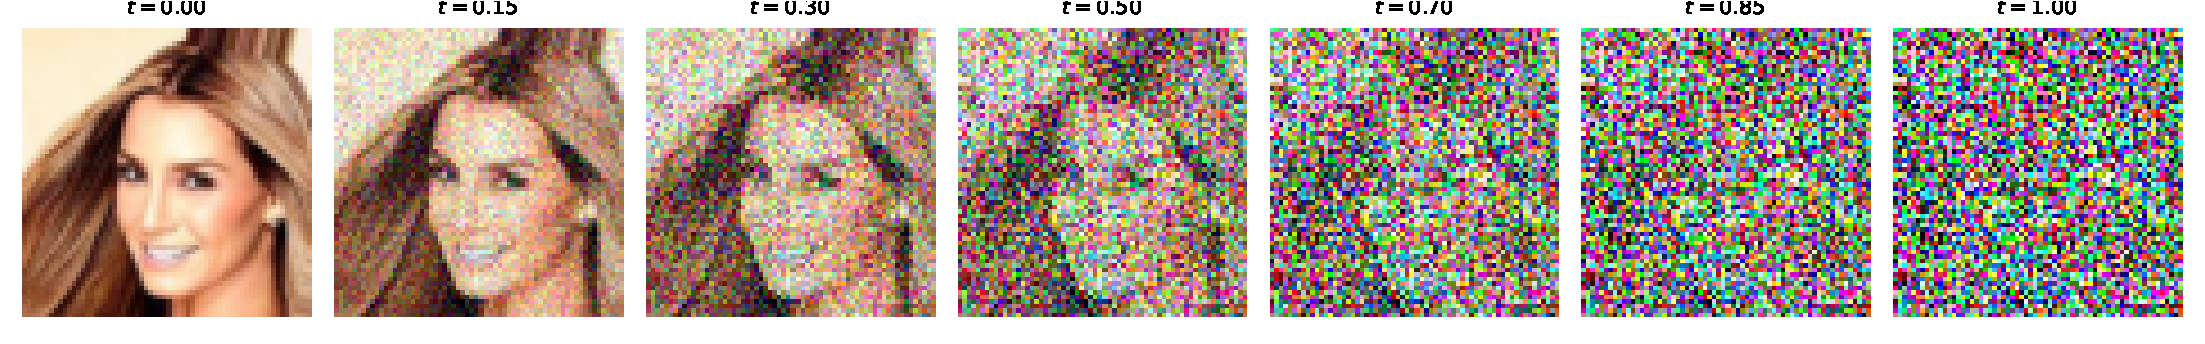
\includegraphics[width=\textwidth]{figures/flow_interpolation.pdf}
\caption{Interpolation linéaire~\eqref{eq:flow-interp} entre une image réelle et un bruit fixé, pour
plusieurs valeurs de $t$. À comparer avec la figure~\ref{fig:forward-diffusion} (bruitage DDPM) : la
dégradation est ici parfaitement régulière et prévisible, puisque déterministe.}
\label{fig:flow-interp}
\end{figure}

\begin{figure}[h]
\centering
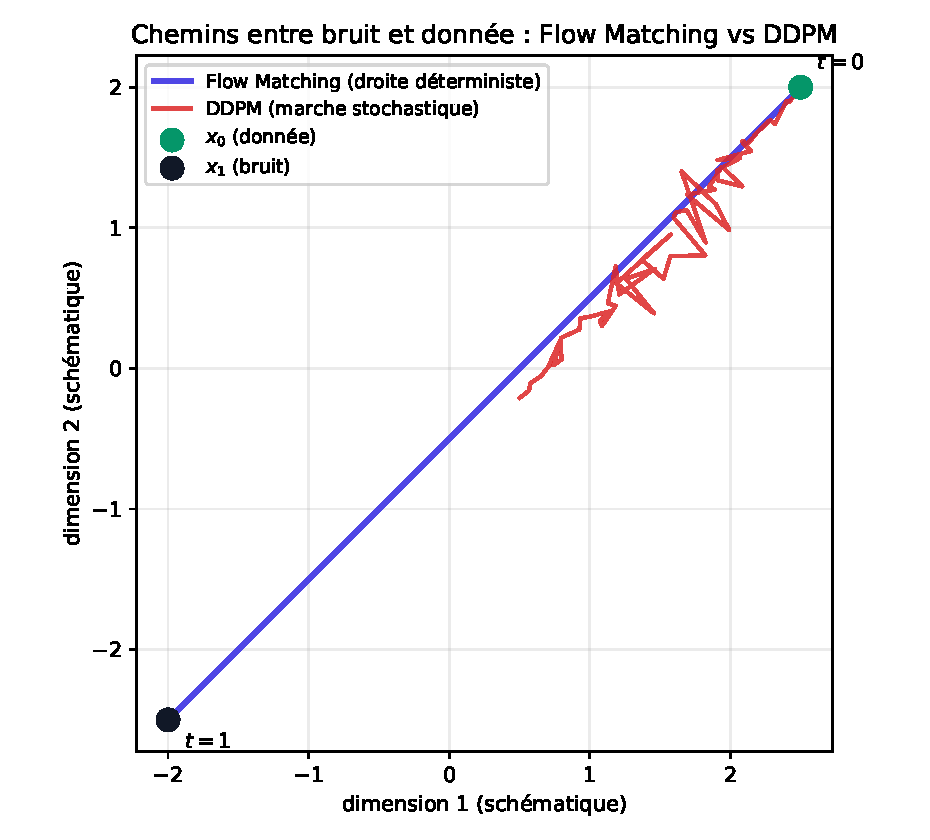
\includegraphics[width=0.72\textwidth]{figures/ddpm_vs_flow_paths.pdf}
\caption{Illustration schématique (exemple jouet en 2D, sans rapport avec le vrai espace des images)
de la différence entre les deux processus : le flow matching suit une trajectoire rectiligne et
déterministe, le DDPM une marche bruitée qui suit le même schedule cumulatif $\bar\alpha_t$ mais avec
des écarts aléatoires à chaque pas.}
\label{fig:paths-comparison}
\end{figure}

\section{Le champ de vitesse}

Dériver l'équation~\eqref{eq:flow-interp} par rapport à $t$ donne la \textbf{vélocité} du point le long
du chemin :
\begin{equation}
    \frac{dx_t}{dt} = x_1 - x_0
\end{equation}
Remarquez que cette quantité ne dépend pas de $t$ : elle est \textbf{constante le long de tout le
segment} — c'est la vitesse d'un mouvement rectiligne uniforme entre $x_0$ et $x_1$.

\begin{definition}[Objectif du flow matching]
On entraîne un réseau $v_\theta(x, t)$ à prédire cette vélocité, pour n'importe quel point $x$ sur
n'importe quel chemin, à n'importe quel instant $t$ :
\begin{equation}
    \boxed{\mathcal{L}_{\text{FM}}(\theta) = \mathbb{E}_{t \sim \mathcal{U}[0,1],\ x_0 \sim p_{\text{data}},\ x_1 \sim \mathcal{N}(0,I)}\left[\left\lVert v_\theta\big((1-t)x_0 + t x_1,\ t\big) - (x_1 - x_0) \right\rVert^2\right]}
\end{equation}
\end{definition}

\begin{intuition}
Chaque paire $(x_0, x_1)$ tirée pendant l'entraînement définit \emph{son propre} segment de droite, de
sa propre vélocité constante $x_1 - x_0$. Le réseau ne voit jamais un segment entier : à chaque exemple
d'entraînement, il ne voit qu'un point $x_t$ tiré sur \emph{un} segment, avec la consigne \og la
vélocité ici doit valoir $x_1 - x_0$ \fg. En moyennant sur des millions de tels segments, le réseau
apprend, pour toute région de l'espace, une vélocité \emph{moyenne} qui tient compte de tous les
segments qui passent à proximité — c'est ce qui permet, à la génération, de suivre un chemin cohérent
même en partant d'un point de bruit qui n'a jamais été vu exactement pendant l'entraînement (voir la
figure~\ref{fig:vector-field}).
\end{intuition}

\begin{figure}[h]
\centering
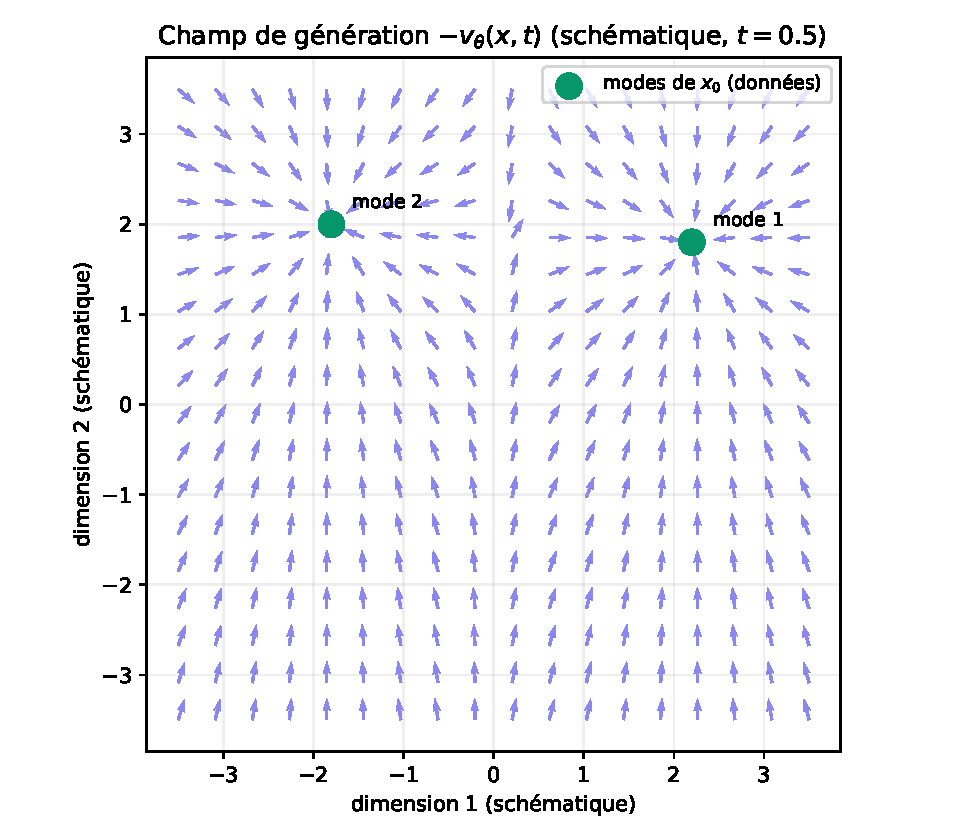
\includegraphics[width=0.7\textwidth]{figures/vector_field.pdf}
\caption{Champ de vitesse appris (schématique, exemple 2D jouet à deux modes de données) : à chaque
point de l'espace, le réseau prédit une direction. Ici on affiche $-v_\theta$, le sens réellement suivi
pendant la génération, qui converge naturellement vers les modes de la distribution de données.}
\label{fig:vector-field}
\end{figure}

\section{Génération : résoudre une équation différentielle}

Une fois $v_\theta$ entraîné, générer une image consiste à résoudre l'équation différentielle ordinaire
\begin{equation}
    \frac{dx_t}{dt} = v_\theta(x_t, t)
\end{equation}
en partant de $x_1 \sim \mathcal{N}(0, I)$ (bruit pur, $t=1$) et en intégrant \textbf{à rebours}
jusqu'à $t=0$. Le schéma numérique le plus simple, l'\textbf{Euler explicite}, discrétise cette
intégration en $N$ pas de taille $dt = 1/N$ :
\begin{equation}
    x_{t - dt} = x_t - dt \cdot v_\theta(x_t, t)
\end{equation}

\begin{codebox}[title=Algorithme : Génération par Flow Matching (Euler explicite)]
\begin{enumerate}[nosep]
    \item tirer $x_1 \sim \mathcal{N}(0, I)$ ; poser $t \leftarrow 1$, $dt \leftarrow 1/N$
    \item \textbf{répéter $N$ fois :}
    \begin{enumerate}[nosep]
        \item calculer $v_\theta(x_t, t)$ avec le réseau entraîné
        \item $x_{t-dt} \leftarrow x_t - dt \cdot v_\theta(x_t, t)$ ; $t \leftarrow t - dt$
    \end{enumerate}
    \item retourner $x_0$
\end{enumerate}
\end{codebox}

\begin{remarque}
Contrairement au reverse process du DDPM (équation~\eqref{eq:psample}), \textbf{aucun bruit aléatoire
n'est réinjecté} à chaque étape : la trajectoire complète est entièrement déterminée par le point de
départ $x_1$ et le réseau $v_\theta$. Deux générations avec le même $x_1$ produisent exactement la
même image. C'est une différence qualitative importante avec le DDPM, dont chaque étape du reverse
process est stochastique.
\end{remarque}

\section{Pourquoi (souvent) moins d'étapes suffisent}

Le chemin appris par le flow matching est, par construction, rectiligne au niveau de chaque exemple
d'entraînement individuel, et le champ moyen résultant tend à rester relativement \og droit \fg. Un
solveur ODE comme Euler explicite approxime d'autant mieux une trajectoire qu'elle est proche d'une
droite : l'erreur de discrétisation d'Euler est en $O(dt)$ par pas, et une trajectoire rectiligne ne
requiert presque aucune correction de direction entre deux pas consécutifs. C'est ce qui explique
pourquoi, en pratique, le flow matching atteint souvent une qualité comparable avec beaucoup moins de
pas de génération ($N \approx 20$–$50$) qu'un DDPM classique ($T \approx 250$–$1000$), bien que ce ne
soit pas une garantie absolue et que cela dépende de la complexité de la distribution de données.

\section{Diffusion et flow matching : une même famille}

Il est utile de noter que DDPM et flow matching, malgré des présentations mathématiques différentes
(chaînes de Markov gaussiennes contre ODE continues), appartiennent tous deux à la famille plus large
des \emph{modèles à transport continu de distribution}, et peuvent même être reliés formellement (le
flow matching avec un chemin gaussien bien choisi retrouve une formulation proche du DDPM en temps
continu). Le tableau~\ref{tab:comparison} résume les différences pratiques entre les deux
implémentations telles qu'utilisées dans ce projet.

\begin{table}[h]
\centering
\begin{tabular}{@{}lll@{}}
\toprule
& \textbf{DDPM} & \textbf{Flow Matching} \\
\midrule
Variable temporelle & $t \in \{0, \dots, T-1\}$ discret & $t \in [0,1]$ continu \\
Construction de $x_t$ & schedule $\bar\alpha_t$ (non-linéaire) & interpolation linéaire \\
Sortie du réseau & bruit $\varepsilon_\theta$ & vélocité $v_\theta$ \\
Cible de la loss & $\varepsilon$ (bruit ajouté) & $x_1 - x_0$ (constant sur le chemin) \\
Génération & stochastique (bruit à chaque pas) & déterministe (ODE) \\
Nb. d'étapes typique & 250 -- 1000 & 20 -- 50 \\
\bottomrule
\end{tabular}
\caption{Comparaison pratique des deux approches implémentées dans ce projet.}
\label{tab:comparison}
\end{table}
